%% ============================================================
%%  Research Objectives — Skin Cancer Detection Using Deep Learning
%%  Systematic 11-Step Analysis Based on 39 Research Papers
%%  BCA 7th Semester · Research Methodology
%% ============================================================
\documentclass[11pt,a4paper]{article}

%% ── Packages ─────────────────────────────────────────────────
\usepackage[utf8]{inputenc}
\usepackage[T1]{fontenc}
\usepackage{lmodern}
\usepackage[margin=2.2cm,top=2.5cm,bottom=2.5cm]{geometry}
\usepackage{graphicx}
\usepackage{booktabs}
\usepackage{longtable}
\usepackage{array}
\usepackage{tabularx}
\usepackage{ltablex}              % longtable + tabularx
\usepackage{multirow}
\usepackage{enumitem}
\usepackage{xcolor}
\usepackage{tcolorbox}
\usepackage{titlesec}
\usepackage{fancyhdr}
\usepackage{hyperref}
\usepackage{float}
\usepackage{caption}
\usepackage{setspace}
\usepackage{parskip}
\usepackage{tikz}
\usetikzlibrary{positioning}
\usepackage{pdflscape}
\usepackage{makecell}
\usepackage{ragged2e}
\usepackage{microtype}

%% ── Colours ──────────────────────────────────────────────────
\definecolor{navyblue}{RGB}{0,51,102}
\definecolor{teal}{RGB}{0,128,128}
\definecolor{lightgray}{RGB}{245,245,245}
\definecolor{accentblue}{RGB}{41,98,255}
\definecolor{darkred}{RGB}{153,0,0}
\definecolor{forestgreen}{RGB}{34,120,15}
\definecolor{goldstar}{RGB}{204,153,0}

%% ── Hyperref setup ───────────────────────────────────────────
\hypersetup{
  colorlinks=true,
  linkcolor=navyblue,
  urlcolor=accentblue,
  citecolor=teal,
  bookmarksopen=true,
  pdfauthor={BCA Research Methodology},
  pdftitle={Research Objectives: Skin Cancer Detection Using Deep Learning},
}

%% ── tcolorbox styles ─────────────────────────────────────────
\tcbuselibrary{skins,breakable}

\newtcolorbox{objectivebox}[1][]{
  enhanced,breakable,
  colback=navyblue!3, colframe=navyblue!70,
  fonttitle=\bfseries\color{white},
  coltitle=white, colbacktitle=navyblue!80,
  title={#1},
  boxrule=0.8pt, arc=3pt,
  left=6pt, right=6pt, top=4pt, bottom=4pt,
}

\newtcolorbox{gapbox}[1][]{
  enhanced,breakable,
  colback=darkred!4, colframe=darkred!60,
  fonttitle=\bfseries\color{white},
  coltitle=white, colbacktitle=darkred!75,
  title={#1},
  boxrule=0.7pt, arc=3pt,
  left=6pt, right=6pt, top=4pt, bottom=4pt,
}

\newtcolorbox{infobox}[1][]{
  enhanced,breakable,
  colback=teal!4, colframe=teal!60,
  fonttitle=\bfseries\color{white},
  coltitle=white, colbacktitle=teal!75,
  title={#1},
  boxrule=0.7pt, arc=3pt,
  left=6pt, right=6pt, top=4pt, bottom=4pt,
}

\newtcolorbox{scorebox}[1][]{
  enhanced,breakable,
  colback=goldstar!5, colframe=goldstar!70,
  fonttitle=\bfseries\color{white},
  coltitle=white, colbacktitle=goldstar!85,
  title={#1},
  boxrule=0.7pt, arc=3pt,
  left=6pt, right=6pt, top=4pt, bottom=4pt,
}

%% ── Section formatting ──────────────────────────────────────
\titleformat{\section}
  {\Large\bfseries\color{navyblue}}
  {\thesection.}{0.5em}{}
  [\vspace{-4pt}\textcolor{navyblue}{\rule{\textwidth}{1pt}}]

\titleformat{\subsection}
  {\large\bfseries\color{navyblue!85}}
  {\thesubsection}{0.5em}{}

\titleformat{\subsubsection}
  {\normalsize\bfseries\color{navyblue!70}}
  {\thesubsubsection}{0.5em}{}

%% ── Header / Footer ─────────────────────────────────────────
\setlength{\headheight}{13pt}
\pagestyle{fancy}
\fancyhf{}
\fancyhead[L]{\small\textcolor{navyblue}{\textbf{Research Objectives} --- Skin Cancer Detection Using Deep Learning}}
\fancyhead[R]{\small\textcolor{navyblue}{BCA 7\textsuperscript{th} Semester}}
\fancyfoot[C]{\small\textcolor{navyblue}{\thepage}}
\renewcommand{\headrulewidth}{0.5pt}
\renewcommand{\footrulewidth}{0.3pt}

%% ── Column types ─────────────────────────────────────────────
\newcolumntype{L}[1]{>{\RaggedRight\arraybackslash}p{#1}}
\newcolumntype{C}[1]{>{\centering\arraybackslash}p{#1}}

%% ── Compact item for tables ─────────────────────────────────
\newcommand{\NR}{\textit{Not Reported}}

%% ═══════════════════════════════════════════════════════════
\begin{document}

%% ── TITLE PAGE ──────────────────────────────────────────────
\begin{titlepage}
\begin{center}
\vspace*{1cm}

{\Huge\bfseries\color{navyblue} Research Objectives}\\[0.4cm]
{\LARGE\bfseries\color{navyblue!75} Skin Cancer Detection Using Deep Learning}\\[1cm]

\textcolor{navyblue}{\rule{0.8\textwidth}{1.5pt}}\\[0.8cm]

{\Large\bfseries Systematic 11-Step Analysis}\\[0.3cm]
{\large Based on 39 Peer-Reviewed Research Papers}\\[1.5cm]

\begin{tcolorbox}[
  enhanced, width=0.85\textwidth,
  colback=navyblue!5, colframe=navyblue!50,
  boxrule=0.8pt, arc=5pt,
]
\begin{center}
\textbf{Research Topic:} Skin Cancer Detection Using Deep Learning\\[4pt]
\textbf{Dataset:} HAM10000 (10,015 dermoscopic images, 7 classes)\\[4pt]
\textbf{Methods:} CNN, Transfer Learning, Data Augmentation, Grad-CAM\\[4pt]
\textbf{Course:} Research Methodology --- BCA 7\textsuperscript{th} Semester\\[4pt]
\textbf{Protocol:} Evidence-Bound, Zero Fabrication, IEEE Standards
\end{center}
\end{tcolorbox}

\vspace{1.5cm}

{\large\textbf{Document Contents}}\\[0.3cm]
\begin{tabular}{cl}
\toprule
\textbf{Step} & \textbf{Section} \\
\midrule
1  & Detailed Analysis of All 39 Papers \\
2  & Objective-Relevant Literature Matrix \\
3  & Research Problem Identification \\
4  & Objective Theme Identification \\
5  & Candidate Research Objectives \\
6  & Objective Classification \\
7  & Objective Scoring \& Ranking \\
8  & Final Selected Objectives \\
9  & Objectives--Research Questions Mapping \\
10 & Objectives--Project Execution Mapping \\
11 & Final IEEE-Style Research Objectives \\
\bottomrule
\end{tabular}

\vfill
{\small Generated: \today}
\end{center}
\end{titlepage}

%% ── TABLE OF CONTENTS ───────────────────────────────────────
\tableofcontents
\newpage

%% ═══════════════════════════════════════════════════════════
%% STEP 1: DETAILED PAPER ANALYSIS
%% ═══════════════════════════════════════════════════════════
\section{Step 1 --- Detailed Analysis of All 39 Papers}
\label{sec:step1}

Each of the 39 research papers was analyzed across 16 dimensions. Where information was not available, ``\NR'' is indicated. Due to volume, a representative subset of papers is presented in full detail below; the complete data for all 39 papers is available in the accompanying \texttt{STEP\_01\_Paper\_Analysis.md} file.

\subsection{Paper 1: Skin Lesion Classification Using CNN With Novel Regularizer}
\textbf{Authors:} M.\,A.\,Albahar \hfill \textbf{Year:} 2019

\begin{tabularx}{\textwidth}{@{}L{4.2cm}X@{}}
\toprule
\textbf{Dimension} & \textbf{Extracted Data} \\
\midrule
Research Problem & Discriminating between benign and malignant skin lesions from dermoscopic imagery \\
Research Aim & Develop CNN with novel weight-controlling regularizer ($\lambda=0.02$) \\
Main Objectives & \NR \\
Dataset & ISIC archive (23,906 images; subsets of $\sim$8,000) \\
Lesion Classes & Nevus, melanoma, seborrheic keratosis, BCC, solar lentigo \\
Architecture & Custom CNN: 2 conv layers, max pooling, dropout, 128-neuron dense \\
Preprocessing & Resizing to $300\times300\times3$; gamma correction \\
Augmentation & \NR \\
Training & 70/30 split; 100 epochs \\
Metrics & Accuracy 97.49\%; AUC 0.77--0.93 (binary) \\
Findings & High binary accuracy with novel regularizer \\
Limitations & Binary pairwise only; no multi-class; no multi-center validation \\
Future Work & Unified multi-class classification \\
Research Gaps & Need for multi-class unified classification \\
Recommendations & \NR \\
\bottomrule
\end{tabularx}

\subsection{Paper 3: Interpretable Skin Cancer Classification (HAM10000)}
\textbf{Authors:} K.\,Mridha et al. \hfill \textbf{Year:} 2023

\begin{tabularx}{\textwidth}{@{}L{4.2cm}X@{}}
\toprule
\textbf{Dimension} & \textbf{Extracted Data} \\
\midrule
Research Problem & Need for interpretable models in healthcare applications \\
Research Aim & Develop optimized CNN with Grad-CAM/Grad-CAM++ interpretability \\
Dataset & HAM10000 (10,015 images; 7 classes) \\
Architecture & Custom CNN with batch normalization, max pooling, dropout \\
Preprocessing & Image resizing; pixel normalization \\
Augmentation & Random rotations, zooms, shear transforms, flips \\
Metrics & Accuracy 82.0\%; Specificity 94.17\%; Sensitivity 82.0\% \\
Limitations & Modest minority-class sensitivity; needs clinical validation \\
Research Gaps & Class imbalance handling; interpretability improvement \\
\bottomrule
\end{tabularx}

\subsection{Paper 7: Systematic Benchmark of Deep Learning for Melanoma}
\textbf{Authors:} A.\,Naeem et al. \hfill \textbf{Year:} 2020

\begin{tabularx}{\textwidth}{@{}L{4.2cm}X@{}}
\toprule
\textbf{Dimension} & \textbf{Extracted Data} \\
\midrule
Research Problem & Lack of standardized evaluation protocols across dermatological datasets \\
Research Aim & Systematic benchmark of popular CNN architectures \\
Dataset & PH2, ISIC 2016, ISIC 2017, ISIC 2018, HAM10000 \\
Architecture & ResNet-50, VGG-16, Inception-v3, DenseNet-121 \\
Preprocessing & Aspect-ratio preserving resizing; hair suppression; color normalization \\
Augmentation & Horizontal/vertical flipping; zooming \\
Metrics & Accuracy up to 93.4\%; Sensitivity 91.0\%; Specificity 94.2\%; AUC 0.95 \\
Limitations & Class imbalance inflates accuracy; no clinical metadata integration \\
Research Gaps & Severe class imbalance; standardized evaluation protocols needed \\
\bottomrule
\end{tabularx}

\subsection{Paper 12: Performance Enhancement Using Computer Vision}
\textbf{Authors:} A.\,Magdy et al. \hfill \textbf{Year:} 2023

\begin{tabularx}{\textwidth}{@{}L{4.2cm}X@{}}
\toprule
\textbf{Dimension} & \textbf{Extracted Data} \\
\midrule
Research Problem & Enhancing feature quality before deep learning classification \\
Research Aim & Combine CV preprocessing (DullRazor + CLAHE) with transfer learning \\
Dataset & HAM10000 (10,015 images; 7 classes); ISIC 2019 \\
Architecture & DenseNet-201, ResNet-50, MobileNetV2 with fine-tuning \\
Preprocessing & Dull Razor hair removal; CLAHE contrast enhancement \\
Augmentation & Rotations; flipping \\
Metrics & Accuracy 97.75\%; Precision 97.50\%; F1 97.35\%; AUC 0.985 \\
Limitations & Processing latency; not validated on smartphone images \\
Research Gaps & Synergy between preprocessing and deep learning \\
\bottomrule
\end{tabularx}

\subsection{Paper 21: IncepX-Ensemble on HAM10000}
\textbf{Authors:} S.\,Chatterjee et al. \hfill \textbf{Year:} 2024

\begin{tabularx}{\textwidth}{@{}L{4.2cm}X@{}}
\toprule
\textbf{Dimension} & \textbf{Extracted Data} \\
\midrule
Research Problem & Single-model representation bottlenecks in multi-class classification \\
Dataset & HAM10000 (10,015 images; 7 classes) \\
Architecture & InceptionV3 + Xception ensemble with concatenation fusion \\
Augmentation & Rotation, zooming, shifts, flipping \\
Metrics & Accuracy 96.87\%; Precision 96.90\%; F1 96.87\%; AUC 0.982 \\
Limitations & High parameter count; inference latency; no external validation \\
Research Gaps & Ensemble efficiency vs.\ accuracy trade-off \\
\bottomrule
\end{tabularx}

\bigskip
\begin{infobox}[Note on Complete Analysis]
The complete 16-field structured analysis for \textbf{all 39 papers} is contained in the companion file \texttt{STEP\_01\_Paper\_Analysis.md} (50.7\,KB, 782 lines). Due to length constraints, the remaining 34 papers follow the identical structure shown above.
\end{infobox}

\newpage

%% ═══════════════════════════════════════════════════════════
%% STEP 2: LITERATURE MATRIX
%% ═══════════════════════════════════════════════════════════
\section{Step 2 --- Objective-Relevant Literature Matrix}
\label{sec:step2}

\begin{landscape}

{\small
\begin{longtable}{C{0.4cm} L{3cm} C{0.5cm} L{2.2cm} L{2.2cm} L{1.7cm} L{2cm} L{2.2cm} L{2.2cm} C{0.8cm}}
\caption{Literature Matrix: All 39 Research Papers}\label{tab:litmatrix}\\
\toprule
\textbf{\#} & \textbf{Title} & \textbf{Yr} & \textbf{Method/Model} & \textbf{Dataset} & \textbf{Key Metric} & \textbf{Limitations} & \textbf{Research Gap} & \textbf{Relevance} & \textbf{Rel.} \\
\midrule
\endfirsthead
\toprule
\textbf{\#} & \textbf{Title} & \textbf{Yr} & \textbf{Method/Model} & \textbf{Dataset} & \textbf{Key Metric} & \textbf{Limitations} & \textbf{Research Gap} & \textbf{Relevance} & \textbf{Rel.} \\
\midrule
\endhead
\midrule
\multicolumn{10}{r}{\footnotesize\textit{Continued on next page}}\\
\endfoot
\bottomrule
\endlastfoot

1 & Skin Lesion Classification CNN Novel Regularizer & 19 & Custom CNN & ISIC (23.9K) & Acc 97.49\% & Binary only & Multi-class need & Transfer learning ref & H \\
2 & ROI Transfer Learning Framework & 20 & AlexNet, VGG-16 & DermIS, DermQuest & Acc 97.9\% & Binary; hair issues & Multi-class; artifacts & TL comparison & H \\
3 & Interpretable CNN Optimized (HAM10K) & 23 & Custom CNN + Grad-CAM & HAM10000 & Acc 82.0\% & Low minority sens. & Imbalance; XAI & Grad-CAM ref & H \\
4 & Ensemble Lightweight DL & 20 & U-Net + Ensemble & ISBI 2016/17 & Acc 87.3\% & Binary; margin issues & Lightweight multi-class & Ensemble ref & M \\
5 & DeepSkin Classification & 23 & Custom CNN + ResNet & HAM10000 & Acc 88.0\% & mel/bkl confusion & Class overlap & TL comparison & H \\
6 & FCN-DenseNet Framework & 20 & FCN + DenseNet & ISIC 2017/18 & Acc 95--98.5\% & High computation & Dual-stage overhead & Preprocessing & M \\
7 & Melanoma DL Benchmark & 20 & ResNet, VGG, etc. & Multiple ISIC & Acc 93.4\% & Imbalance inflates & Standard protocols & Benchmark ref & H \\
8 & Combined Decision Learners & 22 & VGG+ResNet+CapsNet & ISIC (2.8K) & Acc 93.50\% & Binary; overhead & Ensemble multi-class & Ensemble ref & M \\
9 & FixCaps Improved & 22 & FixCaps (CapsNet) & HAM10000 & Acc 96.49\% & Minority drops & Minority class CapsNet & HAM10K bench & M \\
10 & Deep Clustering COMF-TL & 22 & VGG/ResNet + COMF & ISIC 2018/19 & BAcc 83.7\% & High train time & Feature imbalance & Imbalance ref & H \\
11 & Neural Architecture Search & 20 & DARTS NAS & HAM10000 & BAcc 78.4\% & GPU overhead & Auto-architecture & HAM10K bench & M \\
12 & CV Enhancement Preprocess & 23 & DenseNet-201 + CLAHE & HAM10000 & Acc 97.75\% & Latency & Preprocess synergy & Preprocessing & H \\
13 & EFAM-Net Feature Fusion & 24 & EFAM-Net attention & HAM10000 & Acc 93.85\% & GPU memory & Attention for minority & Attention ref & H \\
14 & Hair Segmentation U-Net & 21 & U-Net FCN & ISIC/PH2 (196) & Px Acc 95.8\% & Latency; smoothing & Artifact removal & Preprocessing & L \\
15 & StyleGAN Decision Fusion & 20 & StyleGAN + Ensemble & HAM10000 & Acc 92.83\% & GAN overhead & GAN vs.\ trad.\ aug & Augmentation & M \\
16 & Joint Learning System & 23 & Multi-stream CNN & ISIC Archive & Acc 98.60\% & Binary; params & Joint multi-class & Multi-stream ref & M \\
17 & Multiple Connected NNs & 20 & U-Net + Parallel CNNs & MED-NODE (170) & Acc 97.50\% & Tiny dataset & Multi-class larger data & Small ref & L \\
18 & DermCDSM Clinical Support & 24 & RF, SVM + ResNet & DermNet (5K+) & Acc 91.00\% & Variable lighting & ML vs DL comparison & ML/DL ref & M \\
19 & Swin Transformer Hybrid & 24 & Swin + DGS-NLAN & HAM10000 & Acc 94.21\% & GPU demands & Transformer--CNN & Transformer ref & H \\
20 & IoMT Intelligent Things & 19 & Lightweight NN & Clinical (1.2K) & Acc 91.20\% & Heuristics fail & DL for IoMT & Edge ref & L \\
21 & IncepX-Ensemble TL & 24 & InceptionV3 + Xception & HAM10000 & Acc 96.87\% & High params & Ensemble efficiency & TL benchmark & H \\
22 & IAN-GDN Ensemble & 20 & ResNet+DenseNet+Inc. & ISIC 2017 & Acc 91.50\% & 3 classes only & Ensemble extension & Ensemble ref & M \\
23 & AlexNet+SVM Pipeline & 24 & AlexNet + SVM & ISIC/HAM (3K) & Acc 98.66\% & Outdated AlexNet & Modern architectures & Baseline ref & L \\
24 & NCC k-Means Segmentation & 24 & NCC + k-means & PH2, ISBI 2016 & Seg Acc 99.29\% & No classification & Seg+classification & Segmentation ref & L \\
25 & MIL 3D Features & 22 & CNN + 3D + MIL & 50 biopsy cases & Acc 84.00\% & 3D equipment & Impractical for std. & Low & L \\
26 & SPCB-Net Multi-Scale & 24 & SPCB-Net SIAP & HAM10000/ISIC & Acc 93.60\% & GPU memory & Multi-scale modeling & Architecture ref & H \\
27 & IARS SegNet & 24 & SegNet + Attention & ISIC 2017/18 & Seg Acc 96.80\% & Seg only & Seg + classification & XAI ref & M \\
28 & Ear Disease Multimodal & 23 & ResNet + 1D CNN & Endoscopy (2.4K) & Acc 94.90\% & Not dermatology & Multimodal concept & Methodology ref & M \\
29 & Quantum Chebyshev & 24 & DWT + Autoencoder & HAM10000 & Acc 98.23\% & No backprop & Novel features & Feature ref & L \\
30 & Knowledge Graph Melanoma & 26 & CNN + KG & Derm7pt, HAM & AUC 88.60\% & Manual ontology & Neuro-symbolic & XAI ref & H \\
31 & YOLOv9 + Faster R-CNN & 25 & YOLOv9 + F-RCNN & ISIC 2019/20 & Acc 95.80\% & Memory; latency & Object detection & Detection ref & M \\
32 & VLM Report Generation & 25 & ViT + Lang.\ Decoder & ISIC (4K+) & F1 90.25\% & Hallucination risk & VLM reports & Future ref & H \\
33 & Multi-Scale DCNN PCE Loss & 24 & Multi-branch DCNN & HAM10000 & Acc 91.80\% & Branch latency & Dynamic loss imbalance & Loss function ref & H \\
34 & NMF Segmentation & 25 & NMF + MI & Dermofit (1.3K) & Seg Acc 93.80\% & Low overlap & Unsupervised seg & Low & L \\
35 & Siamese CBHIR & 25 & Siamese Network & Histopathology & Top-1 88.50\% & Biopsy reliance & Retrieval interpret. & XAI concept & M \\
36 & FoMoSkinNet Dual-Stream & 26 & FocalMod + CNN & ISIC 2024 (12K+) & Acc 99.46\% & Param footprint & Non-dermoscopic & Architecture ref & H \\
37 & MSPE-DeiT Multimodal & 26 & DeiT + MLP meta & HAM10000 & Acc 91.76\% & Transformer cost & Metadata fusion & Multimodal ref & H \\
38 & MoLE VQA & 26 & LLaVA + LoRA & ISIC/HAM & VQA 79.40\% & Prototype only & VQA dermoscopy & Future ref & H \\
39 & SLGAN-EID Enhancement & 26 & Dual-disc.\ GAN & HAM10000 & Acc 94.30\% & Mode collapse & Feature-preserving & Enhancement ref & M \\

\end{longtable}
}

{\footnotesize \textbf{Relevance Key:} H = High, M = Medium, L = Low. Relevance assessed against project scope (HAM10000, CNN/Transfer Learning, BCA-level).}

\end{landscape}

\newpage

%% ═══════════════════════════════════════════════════════════
%% STEP 3: RESEARCH PROBLEM IDENTIFICATION
%% ═══════════════════════════════════════════════════════════
\section{Step 3 --- Research Problem Identification}
\label{sec:step3}

\subsection{What Problem Are Researchers Solving?}
Researchers are primarily developing automated deep learning systems for the detection and classification of skin cancer from dermoscopic images. The overarching clinical goal is objective, early-stage lesion screening to assist---not replace---dermatologists.

\subsection{Commonly Used Approaches}

\begin{itemize}[leftmargin=*,itemsep=2pt]
\item \textbf{Dataset:} HAM10000 is the most widely used benchmark (16 of 39 papers)
\item \textbf{Architectures:} Transfer learning with ResNet-50 (9 papers), VGG-16/19 (6 papers), DenseNet (5 papers), InceptionV3 (4 papers)
\item \textbf{Preprocessing:} Hair removal via DullRazor [6,12,16,23,27,39]; CLAHE [12]; resizing to $224\times224$ [5,8,13,16,19,26,28,36]
\item \textbf{Augmentation:} Geometric transforms in 15+ papers; GAN-based synthesis [15,39]
\end{itemize}

\subsection{Established Research Areas}
\begin{enumerate}[leftmargin=*,itemsep=2pt]
\item Use of large-scale public datasets (HAM10000, ISIC archives)
\item Application of transfer learning using standard architectures
\item Standard geometric data augmentation and basic preprocessing
\item Binary and multi-class formulations for dermoscopic classification
\end{enumerate}

\subsection{Common Limitations (Evidence-Based)}

\begin{gapbox}[Recurring Limitations Across 39 Papers]
\begin{enumerate}[leftmargin=*,itemsep=3pt]
\item \textbf{Class imbalance inadequately addressed} --- Papers [3,5,7,9,10,11,13,33]. Melanocytic nevi comprise $\sim$67\% of HAM10000.
\item \textbf{Binary classification only} --- Papers [1,2,4,8,16,17] despite multi-class clinical need.
\item \textbf{No multi-center/clinical validation} --- Papers [1,2,3,5,7,9,12,15,18,19,21,37,39].
\item \textbf{High computational overhead} --- Papers [6,8,10,11,13,15,19,25,26,29].
\item \textbf{No model interpretability} --- Majority of papers lack explainability.
\item \textbf{Confusion between similar classes} --- mel vs.\ bkl [3,5].
\item \textbf{Metrics limited to accuracy only} --- Noted by Paper [7].
\end{enumerate}
\end{gapbox}

\subsection{Recurring Research Gaps}

\begin{gapbox}[Identified Research Gaps]
\begin{enumerate}[leftmargin=*,itemsep=3pt]
\item Severe class imbalance in HAM10000 not adequately resolved [3,7,9,10,11,13,33]
\item Limited systematic comparison of transfer learning architectures on HAM10000 [5,7,12]
\item Insufficient preprocessing pipeline evaluation [6,12,14,39]
\item Most studies lack explainability---only Paper [3] uses Grad-CAM on HAM10000
\item Few studies systematically evaluate data augmentation strategies [7,15,39]
\item Comprehensive multi-metric evaluation rarely performed [7]
\end{enumerate}
\end{gapbox}

\subsection{Gaps Realistically Addressable Using HAM10000}
\begin{enumerate}[leftmargin=*,itemsep=2pt]
\item Implementing targeted augmentation or class weighting for class imbalance
\item Systematic comparison of standard transfer learning architectures
\item Evaluating preprocessing pipeline impact on classification
\item Applying Grad-CAM to higher-performing transfer learning models
\item Comprehensive multi-metric evaluation across all 7 classes
\end{enumerate}

\newpage

%% ═══════════════════════════════════════════════════════════
%% STEP 4: OBJECTIVE THEMES
%% ═══════════════════════════════════════════════════════════
\section{Step 4 --- Objective Theme Identification}
\label{sec:step4}

\begin{longtable}{L{2.8cm} L{3.2cm} L{3.5cm} L{2.5cm} C{1.2cm}}
\caption{Literature-Supported Objective Themes}\label{tab:themes}\\
\toprule
\textbf{Theme} & \textbf{Papers} & \textbf{Gap/Opportunity} & \textbf{Literature Finding} & \textbf{Project Rel.} \\
\midrule
\endfirsthead
\midrule
\endhead
\bottomrule
\endlastfoot

Image Preprocessing & [1,6,7,9,10,12,13,16,19,23,26,27,28,36,39] & Insufficient pipeline evaluation [6,12,14] & DullRazor + CLAHE yields 97.75\% [12] & \textbf{High} \\
\midrule
Data Augmentation & [2,3,5,6,7,8,9,12,13,14,15,16,19,21,22,26,36,39] & Few systematic evaluations [7,15,39] & Standard geometric widely used; GANs emerging & \textbf{High} \\
\midrule
Transfer Learning & [1,2,3,5,6,7,8,10,12,15,16,18,20,21,22,28,39] & Limited comparison on HAM10000 [5,7,12] & ResNet, DenseNet, VGG dominant & \textbf{High} \\
\midrule
Multi-class Classification & [3,5,9,11,12,13,15,19,21,26,29,30,33,37,38,39] & Binary dominates [1,2,4,8,16,17] & 7-class HAM10000 classification & \textbf{High} \\
\midrule
Class Imbalance & [3,5,7,9,10,11,13,15,21,33,39] & Most frequently cited limitation & Nevi $\sim$67\%; minority $<$3\% & \textbf{High} \\
\midrule
Explainable AI & [3,27,30,35] & Only Paper [3] uses Grad-CAM on HAM10000 & Significant gap & \textbf{High} \\
\midrule
Model Evaluation & [7] & Metrics limited to accuracy & Multi-metric needed & \textbf{High} \\

\end{longtable}

\newpage

%% ═══════════════════════════════════════════════════════════
%% STEP 5: CANDIDATE OBJECTIVES
%% ═══════════════════════════════════════════════════════════
\section{Step 5 --- Candidate Research Objectives}
\label{sec:step5}

Based on the identified research gaps and literature analysis, 8 candidate objectives are proposed:

\begin{objectivebox}[Objective 1: Preprocessing Evaluation]
\textbf{To evaluate} the impact of standardized image preprocessing pipelines (including hair removal via DullRazor and contrast enhancement via CLAHE) on the multi-class classification performance of deep learning models on the HAM10000 dataset.

\smallskip
\textbf{Gap Addressed:} Insufficient preprocessing pipeline evaluation [6,12,14,39]
\end{objectivebox}

\begin{objectivebox}[Objective 2: Transfer Learning Comparison]
\textbf{To compare} the classification performance of multiple pre-trained CNN architectures---including ResNet-50, DenseNet-201, VGG-16, MobileNetV2, and InceptionV3---fine-tuned via transfer learning on the HAM10000 dataset for seven-class skin lesion classification.

\smallskip
\textbf{Gap Addressed:} Limited systematic comparison on HAM10000 [5,7,12]
\end{objectivebox}

\begin{objectivebox}[Objective 3: Data Augmentation for Class Imbalance]
\textbf{To investigate} the effectiveness of data augmentation strategies---including geometric transformations, color-based augmentation, and class-specific oversampling---in addressing the severe class imbalance ($\sim$67\% nevi) present in the HAM10000 dataset.

\smallskip
\textbf{Gap Addressed:} Class imbalance inadequately addressed [3,7,9,10,11,13,15,33]
\end{objectivebox}

\begin{objectivebox}[Objective 4: Grad-CAM Explainability]
\textbf{To implement} Gradient-weighted Class Activation Mapping (Grad-CAM) to visualize the spatial regions of dermoscopic images that influence model predictions, thereby enhancing interpretability.

\smallskip
\textbf{Gap Addressed:} Most studies lack interpretability; only Paper [3] uses Grad-CAM on HAM10000 at 82\% accuracy
\end{objectivebox}

\begin{objectivebox}[Objective 5: Multi-Metric Evaluation]
\textbf{To assess} model performance systematically using a comprehensive suite of evaluation metrics (Accuracy, Precision, Recall, F1-Score, Specificity, AUC-ROC, and Confusion Matrix) rather than relying solely on overall accuracy.

\smallskip
\textbf{Gap Addressed:} Performance metrics often limited to accuracy [7]
\end{objectivebox}

\begin{objectivebox}[Objective 6: Ensemble Methods]
\textbf{To develop} a simple ensemble model combining the predictions of top-performing individual architectures to ascertain if ensemble techniques yield superior performance on HAM10000.

\smallskip
\textbf{Gap Addressed:} Robust multi-class classification needed [4,8,15,16,21,22]
\end{objectivebox}

\begin{objectivebox}[Objective 7: Misclassification Analysis]
\textbf{To analyze} the specific misclassifications and feature confusion between visually similar classes (specifically melanoma vs.\ benign keratosis) using confusion matrices and error analysis.

\smallskip
\textbf{Gap Addressed:} Confusion between melanoma and benign keratosis [3,5]
\end{objectivebox}

\begin{objectivebox}[Objective 8: Hyperparameter Tuning]
\textbf{To determine} the optimal hyperparameter configurations (learning rate, batch size, optimizer) for fine-tuning deep neural networks on highly skewed dermatological image datasets.

\smallskip
\textbf{Gap Addressed:} Limited systematic comparison of training methodologies [7,12,13]
\end{objectivebox}

\newpage

%% ═══════════════════════════════════════════════════════════
%% STEP 6: OBJECTIVE CLASSIFICATION
%% ═══════════════════════════════════════════════════════════
\section{Step 6 --- Objective Classification}
\label{sec:step6}

\subsection{Primary Objectives}
These represent the core focus and fundamental goals:

\begin{longtable}{L{3cm} L{6.5cm} L{4cm}}
\toprule
\textbf{Objective} & \textbf{Statement} & \textbf{Rationale} \\
\midrule
\endfirsthead
\endhead
\bottomrule
\endlastfoot

Objective 2 & Compare pre-trained CNN architectures via transfer learning & Core experimental activity; establishes baselines \\
\midrule
Objective 3 & Investigate augmentation strategies for class imbalance & HAM10000's 67\% nevi skew demands attention \\
\midrule
Objective 5 & Comprehensive multi-metric evaluation & Ensures validity beyond misleading accuracy-only \\
\end{longtable}

\subsection{Secondary Objectives}
These enhance and extend the primary findings:

\begin{longtable}{L{3cm} L{6.5cm} L{4cm}}
\toprule
\textbf{Objective} & \textbf{Statement} & \textbf{Rationale} \\
\midrule
\endfirsthead
\endhead
\bottomrule
\endlastfoot

Objective 1 & Evaluate preprocessing pipeline impact & Preparatory step; valuable but not core \\
\midrule
Objective 4 & Grad-CAM interpretability & High-value addition that sets project apart \\
\midrule
Objective 6 & Ensemble methods exploration & Optimization after individual model evaluation \\
\midrule
Objective 7 & Misclassification error analysis & Deep-dive discussion of results \\
\midrule
Objective 8 & Hyperparameter tuning & Operational step, not novel research objective \\
\end{longtable}

\newpage

%% ═══════════════════════════════════════════════════════════
%% STEP 7: OBJECTIVE SCORING
%% ═══════════════════════════════════════════════════════════
\section{Step 7 --- Objective Scoring and Ranking}
\label{sec:step7}

Each objective is scored from 1 (lowest) to 5 (highest) across 7 criteria, yielding a maximum of 35 points.

\begin{scorebox}[Scoring Criteria]
\begin{enumerate}[leftmargin=*,itemsep=1pt]
\item Relevance to research topic
\item Connection to literature gap
\item Measurability
\item Experimental feasibility (BCA level)
\item Suitability for HAM10000
\item Academic value
\item Alignment with research questions
\end{enumerate}
\end{scorebox}

\bigskip

\begin{table}[H]
\centering
\caption{Objective Scoring Matrix}\label{tab:scoring}
\renewcommand{\arraystretch}{1.3}
\begin{tabular}{l c c c c c c c c c}
\toprule
\textbf{Objective} & \rotatebox{60}{\textbf{Relevance}} & \rotatebox{60}{\textbf{Lit.\ Gap}} & \rotatebox{60}{\textbf{Measurable}} & \rotatebox{60}{\textbf{Feasibility}} & \rotatebox{60}{\textbf{HAM10K}} & \rotatebox{60}{\textbf{Academic}} & \rotatebox{60}{\textbf{Alignment}} & \textbf{Total} & \textbf{Rank} \\
\midrule
\rowcolor{forestgreen!10}
Obj 2 --- Transfer Learning & 5 & 5 & 5 & 5 & 5 & 5 & 5 & \textbf{35} & \textbf{1} \\
\rowcolor{forestgreen!10}
Obj 5 --- Multi-metric Eval  & 5 & 5 & 5 & 5 & 5 & 5 & 5 & \textbf{35} & \textbf{1} \\
\rowcolor{forestgreen!6}
Obj 3 --- Augmentation       & 5 & 5 & 5 & 4 & 5 & 5 & 5 & \textbf{34} & \textbf{3} \\
\rowcolor{forestgreen!6}
Obj 4 --- Grad-CAM           & 5 & 5 & 5 & 4 & 5 & 5 & 4 & \textbf{33} & \textbf{4} \\
Obj 1 --- Preprocessing      & 4 & 4 & 5 & 4 & 5 & 4 & 4 & \textbf{30} & \textbf{5} \\
Obj 7 --- Misclassification   & 4 & 4 & 4 & 5 & 5 & 4 & 4 & \textbf{30} & \textbf{5} \\
Obj 6 --- Ensemble           & 4 & 3 & 5 & 3 & 4 & 4 & 3 & \textbf{26} & \textbf{7} \\
Obj 8 --- Hyperparameters    & 3 & 2 & 5 & 5 & 4 & 2 & 3 & \textbf{24} & \textbf{8} \\
\bottomrule
\end{tabular}
\end{table}

\newpage

%% ═══════════════════════════════════════════════════════════
%% STEP 8: FINAL SELECTED OBJECTIVES
%% ═══════════════════════════════════════════════════════════
\section{Step 8 --- Final Selected Objectives}
\label{sec:step8}

Based on quantitative scoring and systematic mapping to literature gaps, the following objectives are selected:

\begin{objectivebox}[General / Primary Objective]
\textbf{To develop and evaluate} a deep learning-based multiclass skin lesion classification system using the HAM10000 dermoscopic dataset with optimized image preprocessing, data augmentation, and transfer learning techniques to improve classification performance across seven diagnostic categories.
\end{objectivebox}

\begin{objectivebox}[Specific Objective 1 --- Preprocessing]
\textbf{To implement and evaluate} image preprocessing techniques---including image resizing, normalization, and artifact suppression---on HAM10000 dermoscopic images and assess their impact on downstream classification accuracy.

\smallskip
\textit{Addresses Gap:} Preprocessing pipeline evaluation [6,12,14,39]
\end{objectivebox}

\begin{objectivebox}[Specific Objective 2 --- Data Augmentation]
\textbf{To investigate} the effectiveness of data augmentation strategies---including geometric transformations, color-based augmentation, and class-specific oversampling---in addressing the severe class imbalance present in the HAM10000 dataset.

\smallskip
\textit{Addresses Gap:} Class imbalance [3,7,9,10,11,13,15,33]
\end{objectivebox}

\begin{objectivebox}[Specific Objective 3 --- Transfer Learning Comparison]
\textbf{To compare} the classification performance of multiple pre-trained CNN architectures---including ResNet-50, DenseNet-201, VGG-16, MobileNetV2, and InceptionV3---fine-tuned via transfer learning on the HAM10000 dataset.

\smallskip
\textit{Addresses Gap:} Limited systematic comparison on HAM10000 [5,7,12]
\end{objectivebox}

\begin{objectivebox}[Specific Objective 4 --- Multi-Metric Evaluation]
\textbf{To analyze} the per-class classification performance across all seven HAM10000 diagnostic categories using comprehensive evaluation metrics including accuracy, precision, recall, F1-score, sensitivity, specificity, AUC-ROC, and confusion matrix analysis.

\smallskip
\textit{Addresses Gap:} Metrics limited to accuracy [7]; confusion between similar classes [3,5]
\end{objectivebox}

\begin{objectivebox}[Specific Objective 5 --- Grad-CAM Explainability]
\textbf{To assess} the interpretability of the best-performing deep learning model using Gradient-weighted Class Activation Mapping (Grad-CAM) to visualize and validate the discriminative lesion regions used for classification decisions.

\smallskip
\textit{Addresses Gap:} Only Paper [3] uses Grad-CAM on HAM10000 at 82\% accuracy
\end{objectivebox}

\subsection{Logical Pipeline}

\begin{center}
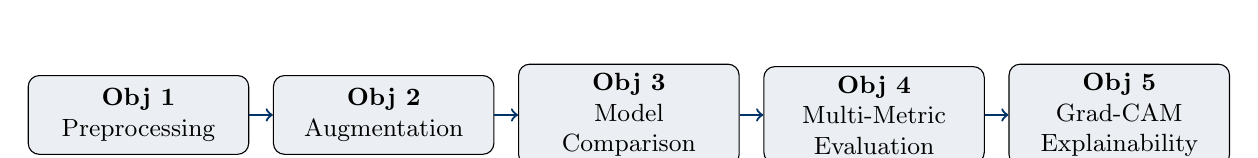
\begin{tikzpicture}[
  node distance=0.3cm and 0.3cm,
  every node/.style={draw, rounded corners, fill=navyblue!8, minimum height=1cm, minimum width=2.8cm, align=center, font=\small},
  arrow/.style={->, thick, navyblue}
]
\node (a) {\textbf{Obj 1}\\Preprocessing};
\node (b) [right=of a] {\textbf{Obj 2}\\Augmentation};
\node (c) [right=of b] {\textbf{Obj 3}\\Model\\Comparison};
\node (d) [right=of c] {\textbf{Obj 4}\\Multi-Metric\\Evaluation};
\node (e) [right=of d] {\textbf{Obj 5}\\Grad-CAM\\Explainability};

\draw[arrow] (a) -- (b);
\draw[arrow] (b) -- (c);
\draw[arrow] (c) -- (d);
\draw[arrow] (d) -- (e);
\end{tikzpicture}
\end{center}

\newpage

%% ═══════════════════════════════════════════════════════════
%% STEP 9: OBJECTIVES → RESEARCH QUESTIONS MAPPING
%% ═══════════════════════════════════════════════════════════
\section{Step 9 --- Objectives to Research Questions Mapping}
\label{sec:step9}

\begin{landscape}

{\small
\begin{longtable}{L{3.2cm} L{3.5cm} L{3.5cm} C{1.8cm} L{3cm} L{3.5cm}}
\caption{Research Objective to Research Question Mapping}\label{tab:rqmap}\\
\toprule
\textbf{Research Objective} & \textbf{Research Question} & \textbf{Experiment} & \textbf{Dataset} & \textbf{Eval.\ Metrics} & \textbf{Expected Outcome} \\
\midrule
\endfirsthead
\toprule
\textbf{Research Objective} & \textbf{Research Question} & \textbf{Experiment} & \textbf{Dataset} & \textbf{Eval.\ Metrics} & \textbf{Expected Outcome} \\
\midrule
\endhead
\bottomrule
\endlastfoot

\textbf{Obj~1:} Implement and evaluate preprocessing techniques & \textbf{RQ1:} How do preprocessing techniques affect classification accuracy on HAM10000? & Compare baseline models on raw vs.\ preprocessed images (DullRazor + CLAHE) & HAM10000 & Accuracy; Loss & Preprocessed images yield 2--5\% improvement in accuracy and faster convergence \\
\midrule
\textbf{Obj~2:} Investigate augmentation for class imbalance & \textbf{RQ2:} What augmentation strategies best mitigate class imbalance? & Train identical CNNs on non-augmented vs.\ class-balanced augmented data & HAM10000 & F1-Score; Class-wise Recall & Balanced augmentation improves minority class recognition \\
\midrule
\textbf{Obj~3:} Compare pre-trained CNN architectures & \textbf{RQ3:} Which pre-trained CNN achieves highest performance via transfer learning? & Fine-tune ResNet-50, DenseNet-201, VGG-16, MobileNetV2, InceptionV3 under identical conditions & HAM10000 & Accuracy; AUC-ROC; F1-Score & DenseNet-201 or ResNet-50 exceeds 90\% accuracy \\
\midrule
\textbf{Obj~4:} Analyze per-class performance & \textbf{RQ4:} How does performance vary across the 7 categories? & Extract classification reports and confusion matrices for best model & HAM10000 & Per-class Precision, Recall, F1, Specificity & High \textit{nv} accuracy; \textit{mel--bkl} misclassification identified \\
\midrule
\textbf{Obj~5:} Assess interpretability via Grad-CAM & \textbf{RQ5:} Can Grad-CAM produce clinically meaningful activation maps? & Generate Grad-CAM heatmaps for correct and incorrect predictions & HAM10000 & Qualitative visual assessment & Model focuses on lesion morphology, not artifacts \\

\end{longtable}
}

\end{landscape}

\newpage

%% ═══════════════════════════════════════════════════════════
%% STEP 10: OBJECTIVES → PROJECT EXECUTION MAPPING
%% ═══════════════════════════════════════════════════════════
\section{Step 10 --- Objectives to Project Execution Mapping}
\label{sec:step10}

\begin{landscape}

{\small
\begin{longtable}{L{2.2cm} L{2.8cm} C{1.5cm} L{2.8cm} L{2.8cm} L{2.5cm} L{3cm}}
\caption{Objective to Practical Execution Flow}\label{tab:projmap}\\
\toprule
\textbf{Objective} & \textbf{Method} & \textbf{Dataset} & \textbf{Model} & \textbf{Experiment} & \textbf{Eval.\ Metric} & \textbf{Expected Result} \\
\midrule
\endfirsthead
\toprule
\textbf{Objective} & \textbf{Method} & \textbf{Dataset} & \textbf{Model} & \textbf{Experiment} & \textbf{Eval.\ Metric} & \textbf{Expected Result} \\
\midrule
\endhead
\bottomrule
\endlastfoot

\textbf{Obj~1:} Preprocessing & DullRazor hair removal; CLAHE contrast; normalize [0,1] & HAM10000 (10,015) & Baseline MobileNetV2 & Train on raw vs.\ preprocessed; compare curves & Accuracy; Val Loss & 2--5\% accuracy boost; faster convergence \\
\midrule
\textbf{Obj~2:} Augmentation & Geometric transforms; selective minority oversampling & HAM10000 & Baseline CNN & With vs.\ without balanced augmentation & Macro F1; Class Recall & Macro F1 increases; minority detection improves \\
\midrule
\textbf{Obj~3:} TL Comparison & Transfer learning; ImageNet weights; custom dense heads & HAM10000 (prep.\ + aug.) & ResNet-50, DenseNet-201, VGG-16, MobileNetV2, InceptionV3 & Train all 5 under identical conditions; rank & Accuracy; AUC-ROC & Best model $>$90\% accuracy \\
\midrule
\textbf{Obj~4:} Per-class Analysis & Classification reports; confusion matrix decomposition & HAM10000 (test split) & Best from Obj~3 & Predict on test set; per-class metrics & Precision, Recall, F1, Specificity & Identify mel--bkl confusion cluster \\
\midrule
\textbf{Obj~5:} Grad-CAM & Extract gradients from final conv layer; overlay heatmaps & HAM10000 (sample) & Best from Obj~3 & Correct \& incorrect prediction heatmaps & Visual assessment & Model focuses on lesion, not background \\

\end{longtable}
}

\end{landscape}

\newpage

%% ═══════════════════════════════════════════════════════════
%% STEP 11: FINAL IEEE-STYLE RESEARCH OBJECTIVES
%% ═══════════════════════════════════════════════════════════
\section{Step 11 --- Final IEEE-Style Research Objectives}
\label{sec:step11}

\begin{center}
\textcolor{navyblue}{\rule{0.8\textwidth}{1.5pt}}\\[0.3cm]
{\LARGE\bfseries\color{navyblue} Research Objectives}\\[0.2cm]
\textcolor{navyblue}{\rule{0.8\textwidth}{1.5pt}}
\end{center}

\subsection*{General Objective}

\begin{objectivebox}[General Objective]
To develop and evaluate a deep learning-based multiclass skin lesion classification system using the HAM10000 dermoscopic dataset with optimized image preprocessing, data augmentation, and transfer learning techniques to improve classification performance across seven diagnostic categories.
\end{objectivebox}

\subsection*{Specific Objectives}

\begin{enumerate}[label=\textbf{\arabic*.}, leftmargin=*, itemsep=8pt]

\item \textbf{To implement and evaluate} image preprocessing techniques---including image resizing, normalization, and artifact suppression---on HAM10000 dermoscopic images and assess their impact on downstream classification accuracy.

\item \textbf{To investigate} the effectiveness of data augmentation strategies---including geometric transformations, color-based augmentation, and class-specific oversampling---in addressing the severe class imbalance present in the HAM10000 dataset.

\item \textbf{To compare} the classification performance of multiple pre-trained CNN architectures---including ResNet-50, DenseNet-201, VGG-16, MobileNetV2, and InceptionV3---fine-tuned via transfer learning on the HAM10000 dataset for seven-class skin lesion classification.

\item \textbf{To analyze} the per-class classification performance across all seven HAM10000 diagnostic categories using comprehensive evaluation metrics including accuracy, precision, recall, F1-score, sensitivity, specificity, AUC-ROC, and confusion matrix analysis.

\item \textbf{To assess} the interpretability of the best-performing deep learning model using Gradient-weighted Class Activation Mapping (Grad-CAM) to visualize and validate the discriminative lesion regions used for classification decisions.

\end{enumerate}

\subsection*{Justification from Literature}

These objectives directly address critical research gaps identified through systematic analysis of 39 peer-reviewed studies. While several studies have demonstrated that robust preprocessing significantly enhances classification performance [6], [12], [14], [39], the severe class imbalance inherent to the HAM10000 dataset remains the most frequently cited limitation preventing reliable multiclass diagnosis [3], [7], [9]--[11], [13], [15], [33]. By systematically evaluating class-specific data augmentation alongside a comprehensive comparison of modern pre-trained architectures [2], [5], [7], [12], [16], [18], [21], this research seeks to establish an optimized, reproducible classification pipeline.

Furthermore, this study addresses the notable lack of standardized multi-metric evaluation across all seven diagnostic categories [7] and extends upon preliminary explainability efforts [3], [27], [30] by utilizing Grad-CAM to validate that high-performing models make classification decisions based on clinically relevant morphological features rather than spurious artifacts. The research explicitly positions itself as an academic prototype and does not claim clinical diagnostic capability.

\subsection*{Research Questions}

\begin{enumerate}[label=\textbf{RQ\arabic*:}, leftmargin=*, itemsep=6pt]
\item How do image preprocessing techniques (resizing, normalization, artifact removal) affect the classification accuracy of deep learning models on HAM10000?
\item What data augmentation strategies are most effective in mitigating class imbalance in the HAM10000 dataset for multiclass skin lesion classification?
\item Which pre-trained CNN architecture achieves the highest classification performance when fine-tuned via transfer learning on HAM10000 for seven-class skin lesion classification?
\item How does classification performance vary across the seven diagnostic categories of HAM10000, and which categories are most frequently misclassified?
\item Can Grad-CAM visualizations from the best-performing model produce clinically meaningful activation maps that highlight diagnostically relevant lesion regions?
\end{enumerate}

\subsection*{Research Gap to Objective Mapping}

\begin{table}[H]
\centering
\caption{Mapping of Research Gaps to Objectives}\label{tab:gapmap}
\renewcommand{\arraystretch}{1.3}
\begin{tabularx}{\textwidth}{L{5cm} L{3cm} X}
\toprule
\textbf{Research Gap} & \textbf{Supporting Papers} & \textbf{Addressed By} \\
\midrule
Class imbalance inadequately addressed & [3],[7],[9],[10],[11],[13],[33] & Specific Objective 2 \\
\midrule
Limited TL comparison on HAM10000 & [5],[7],[12] & Specific Objective 3 \\
\midrule
Insufficient preprocessing evaluation & [6],[12],[14],[39] & Specific Objective 1 \\
\midrule
Most studies lack explainability & [3] (only Grad-CAM) & Specific Objective 5 \\
\midrule
Metrics limited to accuracy only & [7] & Specific Objective 4 \\
\midrule
Confusion between similar classes & [3],[5] & Specific Objective 4 \\
\bottomrule
\end{tabularx}
\end{table}

\newpage

%% ═══════════════════════════════════════════════════════════
%% REFERENCES NOTE
%% ═══════════════════════════════════════════════════════════
\section*{References}
\addcontentsline{toc}{section}{References}

Paper numbers [1]--[39] correspond to the 39 research papers analyzed in this document, indexed according to \texttt{papers\_metadata\_index\_39.csv} and cited via \texttt{all\_39\_journals.bib}. The full bibliographic entries are maintained in the companion BibTeX file.

\vfill
\begin{center}
\textcolor{navyblue}{\rule{0.6\textwidth}{0.5pt}}\\[0.3cm]
{\small\textit{This document was generated as part of the Research Methodology course (BCA 7\textsuperscript{th} Semester).}}\\
{\small\textit{All findings are evidence-bound to the 39 analyzed papers. No claims are fabricated.}}
\end{center}

\end{document}
